
\chapter{Debug Module (DM)} \label{dm}

\begin{steps}{The Debug Module is the interface between specific debug
    operations and their implementation. It might support the following
    operations:}
\item Provide access to a reset signal that allows debugging out of reset.
    (Required)
\item Allow any individual hart to be halted and resumed. (Required)
\item Provide status on which harts are halted. (Required)
\item Provide read and write access to a halted hart's GPRs. (Required)
\item Give the debugger necessary information about the implementation. (Required)
\item Provide access to other hart registers. (Optional)
\item Force the hart to execute arbitrary instructions. (Optional)
\item Allow multiple harts to be halted, resumed, and/or reset at the same time (Optional)
\end{steps}

A single DM can debug up to 1024 harts.

\section{Debug Module Interface (DMI)} \label{dmi}

The Debug Module Interface can be a trivial bus with one master and one slave,
or use a more full-featured bus like TileLink or the AMBA Advanced Peripheral
Bus. The details are left to the system designer.

The DMI uses between 7 and 32 address bits.  It supports read and write
operations, which may return an error. (Errors are only returned by the optional
System Bus Access and Serial Port blocks). The bottom of the address space is
used for the DM. Extra space can be used for custom debug devices, other cores,
additional DMs, etc.

\begin{table}[htp]
    \centering
    \caption{Debug Module Interface Address Space}
    \label{tab:header}
    \begin{tabulary}{\textwidth}{|r|L|}
        \hline
        0x00 -- 0x3f & Registers described in Section~\ref{dmdebbus}. \\
        \hline
        0x40 -- 0x5f & There are 1024 bits here, one for each hart that may
        exist in the system. If the hart is halted, the bit is 1.  Otherwise
        the bit is 0. The bit for hart 0 is the LSB in the 32-bit word at 0x40.
        The bit for hart 1023 is the MSB in the 32-bit word at 0x5f. \\
        \hline
    \end{tabulary}
\end{table}

\section{Reset Control} \label{reset}

This block is connected to a global reset signal, which can
reset, or hold in reset, every component in the platform,
except for the Debug Module and Debug
Transport Modules. The purpose of this feature is to allow debugging
programs from the first instruction executed, so exactly what is affected
by this reset is implementation dependent. Debug Module's own state and registers are
generally reset at power-up and if and only if
\Fdmactive in \Rdmcontrol is 0. This means that the halt state of all harts is
maintained provided that \Fdmactive is 1, although trigger CSRs may be cleared.

\section{Selecting Harts} \label{selectingharts}

Up to 1024 harts can be connected to the DM. The debugger can select any hart
by writing its index to \Fhartsel. Hart indexes start at 0 and are continuous
until the final index. This allows the debugger to enumerate all the harts
attached to the DM by trying each index until \Fanynonexistent is 1.

\section{Halt Control} \label{haltcontrol}

This block controls halt signals from the Debug Module to a hart.  It is used
to halt a hart, and let it run again.

To control halting and resuming, there are \Fhaltreq and \Fresumereq bits in
\Rdmcontrol.  When a debugger wants to halt a hart, it sets \Fhaltreq, waits
for \Fallhalted to indicate the hart is halted, and clears \Fhaltreq.  To
resume, the debugger sets \Fresumereq, waits for \Fallrunning to indicate the
hart is running, and clears \Fresumereq.

The Debug Module conceptually has a direct connection to the halt signal of
every hart that has a halt signal. When set or cleared, a hart must respond in
less than one second.  (How this is implemented is not further specified. A few
clock cycles will be a more typical latency.)

\section{Hart Array Mask Register} \label{hamask}

TODO: Write this section.

\section{Abstract Commands} \label{abstractcommands}

The DM supports a set of abstract commands, which a debugger can execute by
writing the command to \Rcommand.  If the command takes arguments, the debugger
must write them to the {\tt data} registers before writing to \Rcommand. If a
command returns results, they are placed in the {\tt data} registers when the
command is complete. Which {\tt data} registers are used for the arguments is
described in Table~\ref{tab:datareg}.  In all cases the least-significant word
is placed in the lowest-numbered {\tt data} register.  Depending on the
implementation, it may be possible to perform abstract commands even when the
hart is not halted.

\begin{table}[htp]
    \centering
    \caption{Use of Data Registers}
    \label{tab:datareg}
    \begin{tabulary}{\textwidth}{|r|l|l|l|}
        \hline
        XLEN & arg0/return value & arg1 & arg2 \\
        \hline
        32 & \Rdatazero & \Rdataone & \Rdatatwo \\
        \hline
        64 & \Rdatazero, \Rdataone & \Rdatatwo, \Rdatathree & \Rdatafour, \Rdatafive \\
        \hline
        128 & \Rdatazero--\Rdatathree & \Rdatafour--\Rdataseven & \Rdataeight--\Rdataeleven \\
        \hline
    \end{tabulary}
\end{table}

\begin{table}[htp]
    \centering
    \caption{Abstract Register Numbers}
    \label{tab:regno}
    \begin{tabulary}{\textwidth}{|r|l|}
        \hline
        0x0000 -- 0x0fff & CSRs \\
        \hline
        0x1000 -- 0x101f & GPRs \\
        \hline
        0x1020 -- 0x103f & Floating point registers \\
        \hline
        0xc000 -- 0xffff & Reserved for non-standard extensions and internal
        use. \\
        \hline
    \end{tabulary}
\end{table}

\input{abstract_commands.tex}


\begin{figure}
   \centering
   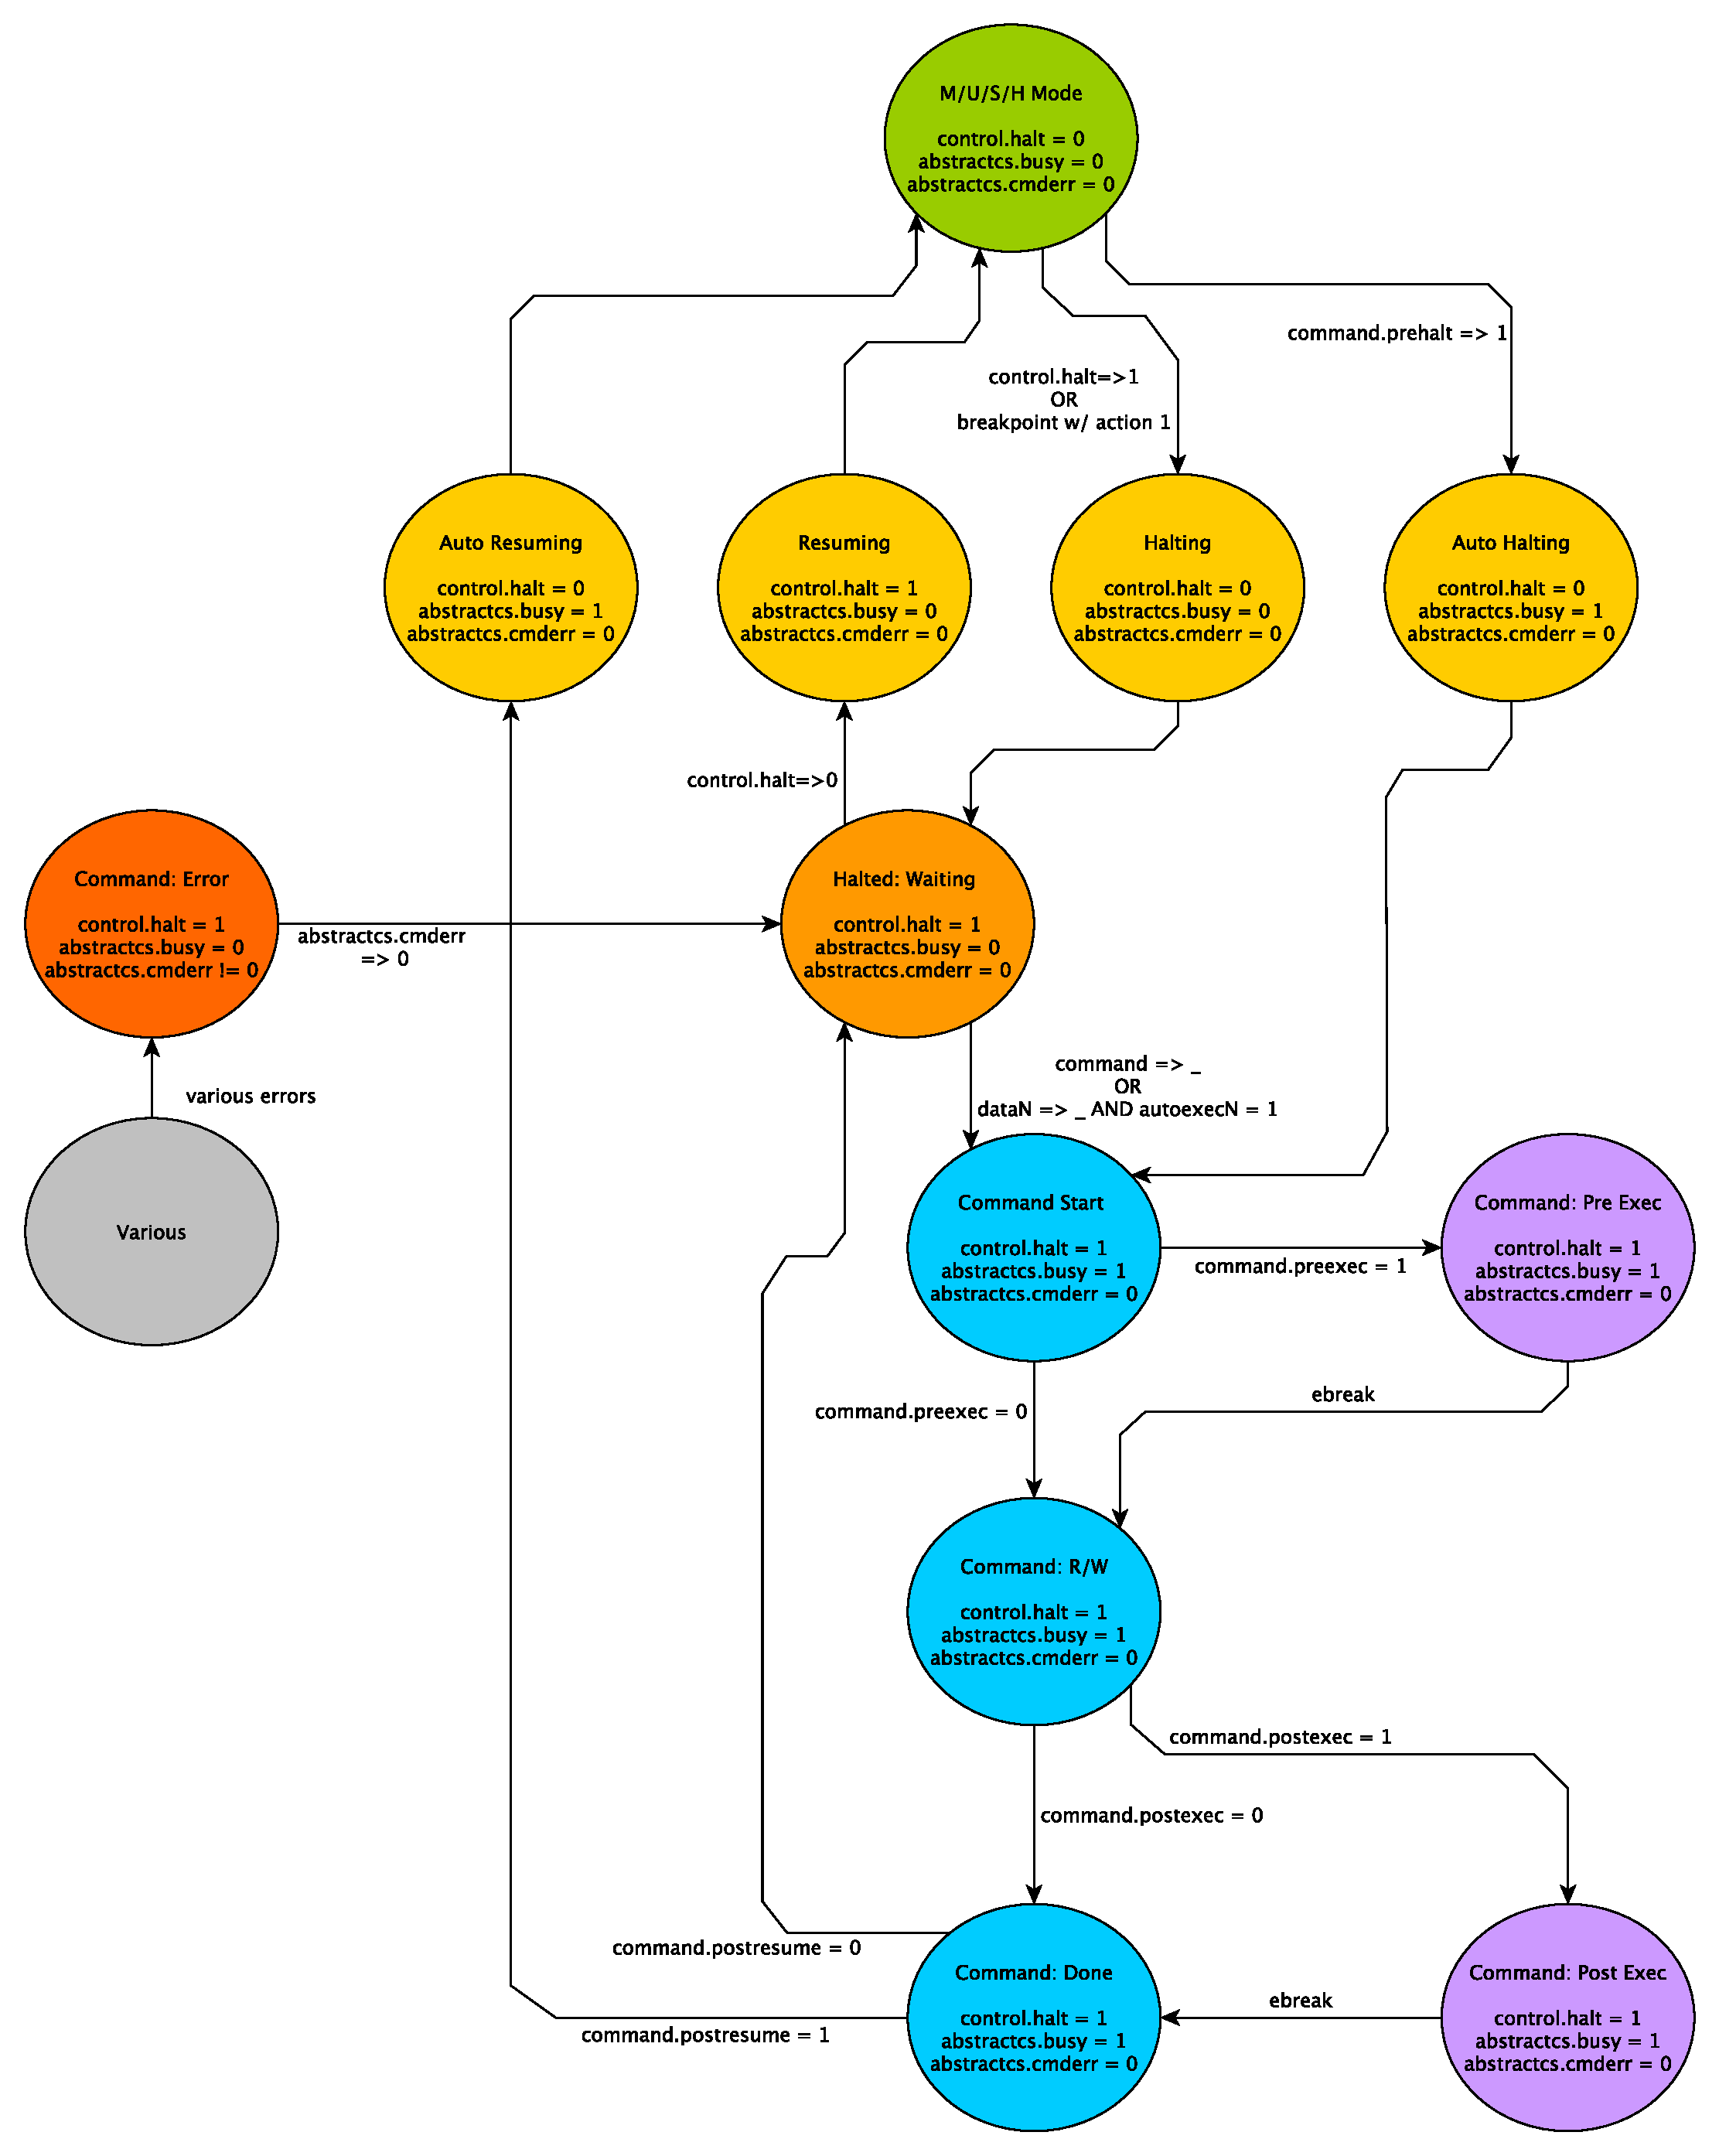
\includegraphics[width=\textwidth]{fig/abstract_commands.pdf}
   \caption[Run/Halt Debug State Machine]{Run/Halt Debug State Machine.
     As only a small amount of state is visibile to the debugger,
     the states and transitions are conceptual.}
   \label{fig:abstract_sm}
\end{figure}

Figure~\ref{fig:abstract_sm} shows a conceptual view of the states
passed through by a hart during run/halt debugging as influenced
by the different fields of \Rcommand.

\section{Program Buffer} \label{programbuffer}

To support executing arbitrary instructions on a halted hart, there may be a
Program Buffer that a debugger can write small programs to. Systems that don't
need any access beyond the abstract commands described in
Section~\ref{abstractcommands} may choose to omit this functionality.

A debugger can write a small program to the optional Program Buffer, and then
execute it exactly once using the \Fpreexec or \Fpostexec bits in \Rcommand.
If \Fprogsize is 1, the Program Buffer may only hold a single instruction.
This can be a 32-bit
instruction, or a compressed instruction in the lower 16 bits accompanied by a
compressed {\tt nop} in the upper 16 bits.  If \Fprogsize is greater than 1,
the debugger can write whatever program it likes, but the program must end with
{\tt ebreak} or {\tt ebreak.c}.

While these programs are executed, the hart does not leave Debug Mode (see
Section~\ref{debugmode}).  If an exception is encountered during execution of
the Program Buffer, no more instructions are executed, the hart remains in Debug
Mode, and \Fcmderr is set to 3.

Executing the Program Buffer may clobber \Rdpc. If that is the case, it must be
possible to read/write \Rdpc using an abstract command. The debugger must
attempt to save \Rdpc between halting and executing a Program Buffer, and then
restore \Rdpc before leaving Debug Mode.

\begin{commentary}
    Allowing Program Buffer execution to clobber \Rdpc allows for direct
    implementations that don't have a separate PC register, and do need to use
    the PC when executing the Program Buffer.
\end{commentary}

\section{System Bus Access} \label{systembusaccess}

When a Program Buffer is present, a debugger can access the system bus by having a
RISC-V hart perform the accesses it requires.
An alternative is to implement a System Bus Access block.
The System Bus Access block uses physical addresses.

\begin{commentary}
Implementing a System Bus Access block has several benefits even
when a Debug Module also implements a Program Buffer. 
First, it is possible to
access memory in a running system with minimal impact.  Second, it may improve
performance when accessing memory.
Third, it may provide
access to devices that a hart does not have access to.
\end{commentary}

\section{Quick Access}

Some systems can only be halted very briefly. There are several mechanisms that
can still allow accessing resources in such a running system.

First, an implementation may implement abstract commands that work without
halting the hart.

Second, the Quick Access abstract command can be used to halt a hart, quickly
execute the contents of the Program Buffer, and let the hart run again.
Combined with instructions that allow Program Buffer code to access the
{\tt data} registers, as described in \ref{hartinfo}, this can be used to quickly
perform a memory or register access. For some systems this will be too
intrusive, but many systems that can't be halted can bear an occasional hiccup
of a hundred or less cycles.

Third, if the System Bus Access block is implemented, it can be used while a
hart is running to access memory.

\section{Security}

To protect intellectual property it may be desirable to lock access to the
Debug Module.  To allow access during a manufacturing process and not
afterwards, a reasonable solution could be to add a fuse bit to the Debug
Module that can be used to be permanently disable it. Since this is technology
specific, it is not further addressed in this spec.

Another option is to allow the DM to be unlocked only by users who have an
access key. A few bits in \Rdmstatus and \Rauthdata can support an arbitrarily
complex authentication mechanism.  When \Fauthenticated is clear, the DM must
not interact with the rest of the platform in any way.

\section{Serial Ports}

The Debug Module may implement up to 8 serial ports. They support basic flow
control and full duplex data transfer between a component and the debugger.
They can be used to communicate with a debug monitor running on a hart, for the
equivalent of printf debugging, to provide a simple CLI without requiring any
extra peripherals, or more generally to emulate devices that aren't present.
All these uses require software support, and are not further specified here.

\section{Debug Module DMI Registers} \label{dmdebbus}

\input{dm1_registers.tex}

\section{Debug Module Serial Registers} \label{dmsysbus}

The Debug Module's serial port registers must be accessible from the
component memory space. The Debug Module's system bus registers  base address
is discoverable in the configuration string. The offsets from this base
are given in this section.

\input{dm2_registers.tex}
